\newpage

\section{Κεφάλαιο 5: Μοτίβα σχεδιασμού και ανθεκτικότητα εφαρμογής}

Η αυτοματοποίηση της ανάπτυξης που περιγράφηκε στα προηγούμενα κεφάλαια διασφαλίζει ότι ο κώδικας φτάνει στο \textit{cluster} με αξιόπιστο και ελεγμένο τρόπο. Το παρόν κεφάλαιο εξετάζει τι περιέχει αυτός ο κώδικας: τα σχεδιαστικά πρότυπα (\textit{design patterns}) που τον καθιστούν ανθεκτικό σε αναμενόμενες αστοχίες --- αποτυχημένες συνδέσεις, διπλά αιτήματα, μεταφορά μεγάλου όγκου δεδομένων --- χωρίς να απαιτείται η παρέμβαση διαχειριστή για κάθε τέτοιο σφάλμα. Σκοπός των επόμενων ενοτήτων είναι να παρουσιάσουν τον κώδικα της εφαρμογής που την κάνει \textit{«άθραυστη»} (\textit{resilient}): ικανή να συνεχίσει να λειτουργεί ορθά παρά τις αναπόφευκτες, μερικές αστοχίες ενός κατανεμημένου συστήματος.

\subsection{\textit{Claim Check Pattern}}

Οι ουρές μηνυμάτων, όπως το \textit{RabbitMQ}, είναι σχεδιασμένες για τη μεταφορά μικρών, ελαφρών μηνυμάτων --- όχι μεγάλων αρχείων. Η απευθείας ενσωμάτωση μιας εικόνας μέσα στο μήνυμα προς το \textit{RabbitMQ} θα επιβάρυνε σημαντικά την ουρά, θα μείωνε την ταχύτητα επεξεργασίας, και θα αύξανε τον κίνδυνο αποτυχίας μεταφοράς για μεγάλα αρχεία.

Το μοτίβο \textit{Claim Check} αντιμετωπίζει αυτό το πρόβλημα διαχωρίζοντας τη μεταφορά του περιεχομένου από τη μεταφορά της \textit{ειδοποίησης}: το αρχείο αποθηκεύεται απευθείας σε εξειδικευμένο αποθηκευτικό χώρο (\textit{MinIO}), και μόνο μια ελαφριά αναφορά --- το \textit{URL} του αποθηκευμένου αντικειμένου --- περνάει μέσα στο μήνυμα προς το \textit{RabbitMQ} και αποθηκεύεται στη βάση δεδομένων:

\begin{lstlisting}[language=yaml, caption={JavaScript συνάρτηση για ανέβασμα αρχείου στο MinIO και επιστροφή του claim check}]
async function uploadAndGetClaimCheck(minioClient, bucket, file, prefix, vmIp) {
  const fileName = `${prefix}-${Date.now()}-${file.originalname}`;
  await minioClient.fPutObject(bucket, fileName, file.path);
  fs.unlinkSync(file.path);
  return `http://${vmIp}:9000/${bucket}/${fileName}`;
}
\end{lstlisting}

Η συνάρτηση αυτή χρησιμοποιείται τόσο για την εικόνα όσο και για το παραστατικό (\textit{invoice}) ενός προϊόντος, επιστρέφοντας σε κάθε περίπτωση μόνο το \textit{URL} αναφοράς --- την «απόδειξη παραλαβής» (\textit{claim check}) --- που χρειάζεται οποιοδήποτε σύστημα κατάντη (\textit{downstream}) για να ανακτήσει το πραγματικό αρχείο, όταν και αν αυτό χρειαστεί.

\newpage

\subsection{\textit{Retry Pattern}}

Κατά την εκκίνηση του \textit{backend container}, η σύνδεση με την εξωτερική βάση δεδομένων (\textit{MongoDB Atlas}) μπορεί να αποτύχει προσωρινά --- για παράδειγμα, λόγω καθυστέρησης στην ετοιμότητα του δικτύου του \textit{cluster}, ή στιγμιαίας μη διαθεσιμότητας της υπηρεσίας. Χωρίς μηχανισμό αντιμετώπισης, μια τέτοια προσωρινή αποτυχία θα οδηγούσε σε πλήρη διακοπή του \textit{pod}, απαιτώντας χειροκίνητη επανεκκίνηση.


Το μοτίβο \textit{Retry} αντιμετωπίζει αυτή την περίπτωση επαναλαμβάνοντας την προσπάθεια σύνδεσης πεπερασμένο αριθμό φορών, με σταθερό χρονικό διάστημα αναμονής μεταξύ των προσπαθειών, πριν αναγνωρίσει οριστική αποτυχία:


\begin{lstlisting}[language=yaml, caption={JavaScript συνάρτηση retryWithDelay για ανθεκτικότητα στο σύστημα}]
async function retryWithDelay(fn, { retries = 3, delayMs = 2000, label } = {}) {
  for (let attempt = 1; attempt <= retries; attempt++) {
    try {
      return await fn();
    } catch (err) {
      if (attempt < retries) {
        await new Promise(resolve => setTimeout(resolve, delayMs));
      } else {
        throw err;
      }
    }
  }
}
\end{lstlisting}

Η συνάρτηση είναι σχεδιασμένη ως γενικευμένο, επαναχρησιμοποιήσιμο εργαλείο (δέχεται οποιαδήποτε ασύγχρονη λειτουργία ως παράμετρο), και όχι ως λογική αποκλειστικά συνδεδεμένη με τη \textit{MongoDB}. Στο σύστημα, χρησιμοποιείται για τη σύνδεση με τη βάση δεδομένων κατά την εκκίνηση, με τρεις προσπάθειες και διάστημα δύο δευτερολέπτων μεταξύ τους.

\subsection{\textit{Idempotency Pattern}}

Σε διεπαφές χρήστη που εμπλέκουν υποβολή φόρμας με μεταφόρτωση αρχείου, είναι σύνηθες φαινόμενο η αθέλητη διπλή υποβολή --- για παράδειγμα, λόγω καθυστέρησης απόκρισης του διακομιστή και επανειλημμένου πατήματος του κουμπιού υποβολής από τον χρήστη. Χωρίς προστασία, κάθε υποβολή θα δημιουργούσε ξεχωριστή εγγραφή στη βάση δεδομένων, παράγοντας διπλά προϊόντα.

Το μοτίβο \textit{Idempotency} αντιμετωπίζει αυτό το πρόβλημα απαιτώντας από τον \textit{client} να αποστείλει ένα μοναδικό κλειδί (\textit{idempotency key}) μαζί με κάθε αίτημα. Ο \textit{server} διατηρεί τα κλειδιά που έχει ήδη επεξεργαστεί, και απορρίπτει άμεσα οποιοδήποτε αίτημα με κλειδί που έχει ξαναχρησιμοποιηθεί:

\newpage

\begin{lstlisting}[language=yaml, caption={Έλεγχος Idempotency για την αποφυγή διπλότυπων αιτημάτων}]
const idempotencyKey = req.body.idempotencyKey;
const { duplicate } = checkIdempotency(idempotencyKey);
if (duplicate) {
  return res.status(409).json({ message: "Duplicate request - product already submitted" });
}
\end{lstlisting}

Η ορθότητα της υλοποίησης επιβεβαιώνεται μέσω αυτοματοποιημένων μοναδιαίων ελέγχων (\textit{unit tests}), που εξετάζουν τρία σενάρια: αίτημα με νέο κλειδί (δεν πρέπει να αναγνωριστεί ως διπλό), αίτημα με ήδη χρησιμοποιημένο κλειδί (πρέπει να αναγνωριστεί ως διπλό), και αίτημα χωρίς κλειδί (δεν πρέπει ποτέ να αναγνωριστεί ως διπλό, καθώς δεν υπάρχει κλειδί προς σύγκριση).

Η συμπεριφορά αυτή επιβεβαιώνεται και σε πραγματικές συνθήκες, πέρα από το περιβάλλον των αυτοματοποιημένων ελέγχων: όπως φαίνεται στην \autoref{fig:idempotency-curl}, ένα πρώτο αίτημα \texttt{POST} με συγκεκριμένο \textit{idempotency key} δημιουργεί επιτυχώς το προϊόν, ενώ ένα δεύτερο, πανομοιότυπο αίτημα με το \textit{ίδιο} κλειδί απορρίπτεται άμεσα με κωδικό κατάστασης \texttt{409 Conflict}, χωρίς να δημιουργηθεί δεύτερη εγγραφή στη βάση δεδομένων.

\begin{figure}[h]
  \centering
  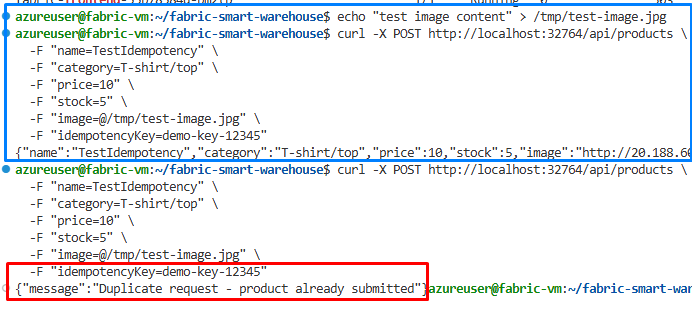
\includegraphics[width=\textwidth]{project/report/figures/idempotency-blocked-req.png}
  \caption{Δοκιμή του \textit{Idempotency Pattern} μέσω \texttt{curl}: το δεύτερο αίτημα με το ίδιο \textit{idempotency key} απορρίπτεται με \texttt{409 Conflict}}
  \label{fig:idempotency-curl}
\end{figure}

\subsection{\textit{Stateless Pattern}}

Σε αντίθεση με τα τρία προηγούμενα μοτίβα, η στατελής (\textit{stateless}) φύση του \textit{backend} δεν εντοπίζεται σε ένα συγκεκριμένο τμήμα κώδικα, αλλά αποτελεί ιδιότητα της συνολικής αρχιτεκτονικής του: ο \textit{server} δεν διατηρεί καμία πληροφορία συνεδρίας (\textit{session}) στη μνήμη του μεταξύ διαδοχικών αιτημάτων. Η αυθεντικοποίηση του χρήστη βασίζεται σε \textit{JSON Web Tokens} (\textit{JWT}), τα οποία μεταφέρουν την απαραίτητη πληροφορία ταυτότητας μέσα στο ίδιο το αίτημα, και κάθε δεδομένο που πρέπει να διατηρηθεί αποθηκεύεται μόνιμα στη \textit{MongoDB}, όχι στη μνήμη του \textit{process}.

Η ιδιότητα αυτή είναι προαπαιτούμενο για την οριζόντια κλιμάκωση (\textit{horizontal scaling}) του \textit{backend}: επειδή κανένα αντίτυπο (\textit{replica}) δεν διατηρεί τοπική κατάσταση, οποιοδήποτε αντίτυπο μπορεί να εξυπηρετήσει οποιοδήποτε αίτημα, χωρίς ανάγκη \textit{«κολλώδους» σύνδεσης} (\textit{sticky session}) μεταξύ συγκεκριμένου χρήστη και συγκεκριμένου αντιτύπου. Αυτό επιτρέπει στο \textit{Horizontal Pod Autoscaler} (\textit{HPA}) που έχει ρυθμιστεί για το \textit{backend} να αυξάνει ή να μειώνει δυναμικά τον αριθμό των αντιτύπων με βάση τον φόρτο, χωρίς κίνδυνο απώλειας πληροφορίας ή ασυνέπειας μεταξύ χρηστών.


Τα σχεδιαστικά πρότυπα που παρουσιάστηκαν --- η αποσύνδεση μεγάλου περιεχομένου από τα μηνύματα, η ανθεκτικότητα σε προσωρινές αποτυχίες δικτύου, η προστασία από διπλές εγγραφές, και η στατελής φύση του \textit{backend} --- δεν λειτουργούν μεμονωμένα, αλλά συνθέτουν ένα σύστημα που παραμένει λειτουργικό υπό συνθήκες που, σε διαφορετική περίπτωση, θα οδηγούσαν σε σφάλματα ή ασυνέπειες δεδομένων. Το επόμενο κεφάλαιο εξετάζει ένα ακόμη τμήμα του συστήματος που υλοποιεί διαφορετική φιλοσοφία υπολογισμού: τη \textit{serverless} εκτέλεση κώδικα, ενεργοποιούμενη αποκλειστικά από συγκεκριμένα γεγονότα.